%%%%%%%%%%%%%%%%%%%%% Current work %%%%%%%%%%%%%%%%%%%%%%%%%%%%%%%%%%%%%

\section{Current work}

\begin{figure}[!th]
    \centering
    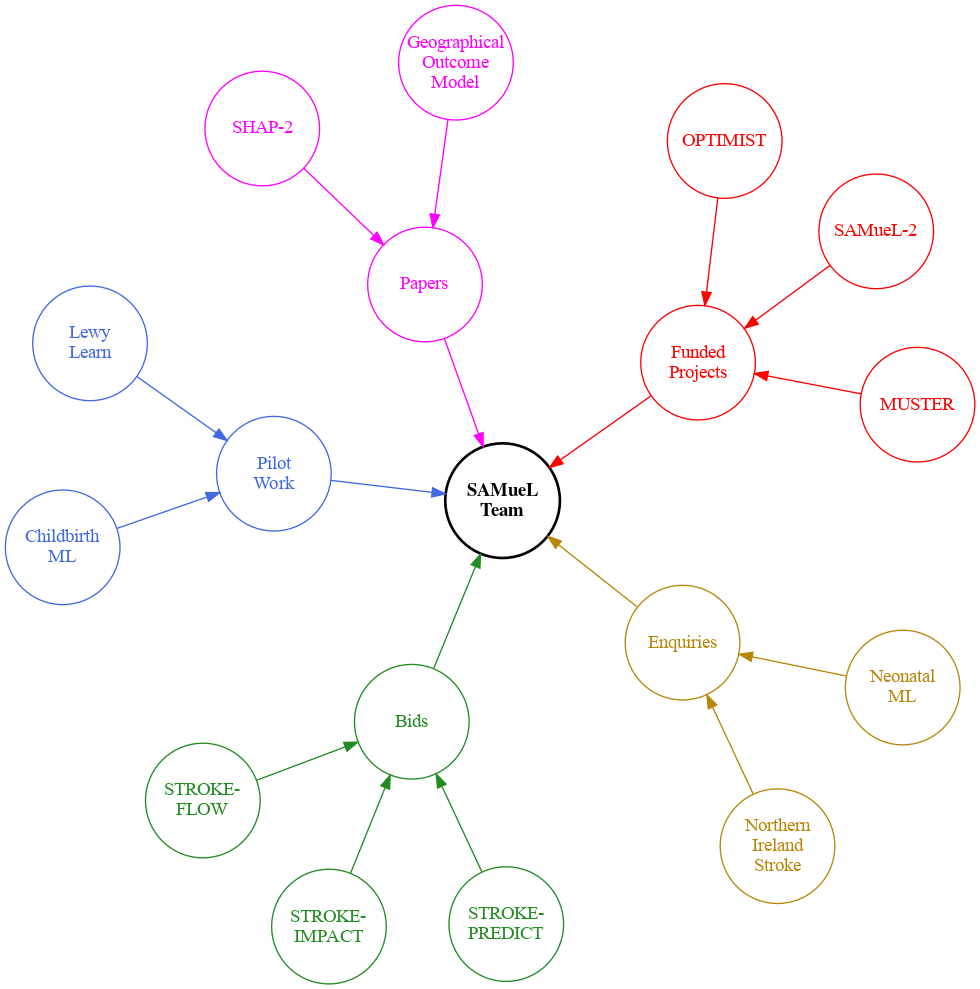
\includegraphics[width=0.8\textwidth]{./images/work}
    \caption{`Stroke Team' Overview - Current Work (August 2023)}
  \label{fig:shap_multiple_regression}
\end{figure}

\subsection{Funded work}

\begin{itemize}
    \item \textbf{SAMueL-2} (Stroke Audit Machine Learning). April 2022 to end July 2024. Nominal funding: MJA 25\%, KP 30\%, AL 100\% (currently being adjusted to fund extension). NIHR Health Services and Delivery Research Reference NIHR134326. £589k. Brief description: Using clinical pathway simulation to model the potential benefit of improving the emergency stroke pathway, and using machine learning to compare clinical decision-making around thrombolysis between hospitals. T1: 119149
    \item \textbf{OPTIMIST} (OPTimising IMplementation of Ischaemic Stroke Thrombectomy). Aug 2021 to end July 2026. Nominal funding: MJA 10\% throughout, AL: 100\% from August 2023 to end July 2026. NIHR Programme Grants for Applied Research NIHR202361: £1.983M. Brief description: Optimising the pre-hospital stroke way to maximise the benefit of thrombolysis and thrombectomy. T1: 116323
    \item \textbf{MUSTER} (Modelling mobile stroke Units for Stroke Treatment Equity and Resources) June 2023 to end November 2024. Nominal funding: MJA 30\%, KP 70\%. NIHR Health Services and Delivery Research Reference NIHR153982. £539k. Brief description: Modelling the resource requirements for implementation of mobile stroke units across the National Health Service, their cost-effectiveness, and their effect on equity of access to emergency stroke care. T1: 122573
\end{itemize}

\subsection{Bids}

\subsubsection{Submitted bids}

\begin{itemize}
    \item \textbf{STROKE-PREDICT}: Using Explainable Artificial Intelligence to predict future stroke using routine historical investigations: 20\% FTE October 2023 for 18 months. \url{https://www.ukri.org/opportunity/artificial-intelligence-innovation-to-accelerate-health-research/} Worktribe ref: 1837420. Funder: EPSCR. Start (if funded) October 2023. Also, similar bid, with MJA for 10\% for 2 years. MRC Call:  \url{https://www.ukri.org/opportunity/funding-for-early-stage-development-of-new-healthcare-interventions/ Worktribe 3177307}
\end{itemize}

\subsubsection{Bids due for September submission}

\begin{itemize}
    \item \textbf{STOKE-IMPACT}: Understanding the impact of clinical practice variation on patient outcomes using explainable machine learning coupled with clinical trial emulation and causal inference studies. A study using national clinical audit data. \url{https://www.nihr.ac.uk/funding/rfpb-under-represented-disciplines-and-specialisms-highlight-notice-methodologists/33231} Expression of interest (500 words) 16 August 2023 at 1pm. Stage 1 13th September. Approx resourcing: KP 50\%, MJA 25\%. Aim to start September 2024. £250K Worktribe: 2692263
    \item \textbf{STROKE-FLOW}: Using explainable machine learning and clinical pathway simulation to model and optimise flow and capacity planning in the in-patient stroke pathway. \url{https://www.nihr.ac.uk/funding/2310-health-and-social-care-delivery-research-programme-researcher-led/32515}. Approx resourcing: New ARF 100\%, KP 30\%, MJA 20\%. Stage 1 deadline: 1pm, 20 September 2023. £500K? Aim to start August 2024. Worktribe: 3020267
\end{itemize}

\subsection{Pilot work}

\begin{itemize}
    \item \textbf{Childbirth-ML}: Predicting interventions and outcome in childbirth. Data source identified for pilot work.
    
    \item \textbf{LewyLearn}: Applying explainable machine learning to investigate variation in diagnosis of dementia with Lewy Bodies. Pilot work on the use of explainable machine learning to analyze the variation in diagnosis rates for dementia with Lewy bodies (DLB) in the National Alzheimer’s Coordinating Center (NACC) Uniform Data Set.
    
\end{itemize}

\subsection{Current resources}

The stroke team currently comprises:

\begin{itemize}
    \item Michael Allen (100\%)
    \item Kerry Pearn (100\%)
    \item Anna Laws (100\%)
    \item Amy Heather (50\%)
\end{itemize}

\begin{minipage}{\textwidth}
\begin{longtable}[]{@{}lll@{}}
\caption{Current allocation of resources to projects}\\
\toprule()
Project & Type & Who? \\
\midrule
SAMueL-2 & Funded work & Kerry, Mike, Anna, Amy \\
OPTIMIST & Funded work & Anna, Mike \\
MUSTER & Funded work & Anna, Mike \\
\midrule
STROKE-IMPACT & Bid & Mike, Kerry \\
STROKE-FLOW & Bid & Mike, Kerry \\
STROKE-PREDICT & Bid & Mike \\
\midrule
Childbirth ML & Pilot work & Mike \\
Lewy Learn & Pilot work & Mike, Kerry \\
\midrule
SHAP-2 & Paper & Kerry, Mike \\
Geographic stroke outcome & Paper & Mike, Anna \\
\midrule
Neonatal ML & Enquiry & None \\
Northern Ireland stoke organisation & Enquiry & None \\
\bottomrule()
\label{tab:resources}
\end{longtable}
\end{minipage}